\documentclass[border=0pt]{standalone}
\usepackage{tikz}
\usepackage{amsmath, amsthm, amssymb}
%\input{commondefinitions}
\usetikzlibrary{plotmarks}
\newcommand\marksymbol[2]{\tikz[#2,scale=1.2]\pgfuseplotmark{#1};}

\newcommand{\mcE}{\mathcal{E}}
\colorlet{coscolor}{blue}

\begin{document}
\newcommand{\tmp}{-4}
\pagestyle{empty}
\begin{tikzpicture} 
%     \node at (0,  0)  {\includegraphics{gamma_sigma}};
%     \node at (0,-2.6) {\footnotesize $n$};
%     \node at (2.6,.15) {\footnotesize $n$};
%     \node at (.7,-1.1) {\rotatebox{90}{\footnotesize $\log_{10} \sigma$}};
%     \node at (0,-2.4) {$\eta$};
%   \node[rotate=90] at (-4.2,0.0) {\footnotesize  $\log_{10} [-\log_{10}(V_\mcE/V_0)]$};
%   \node[rotate=90] at (-4.2,0.0) {\footnotesize  $\log [-\log(V_0/V)]$};
%     \node at (2.2,1.05) [anchor=west] {\rotatebox{20}{\footnotesize $p=0.99$}};
%     \node at (2.2,2.15) [anchor=west] {\rotatebox{20}{\footnotesize $p=0.4$}};
%     \node at (-3.2,2.4) [anchor=west] {\footnotesize Random channel};
    \node at (0,0)         {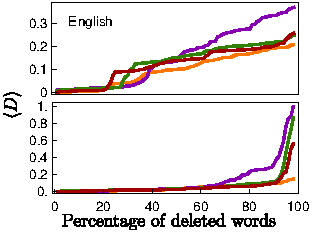
\includegraphics{ds1.pdf}};
    \node at (1*5.2,0)     {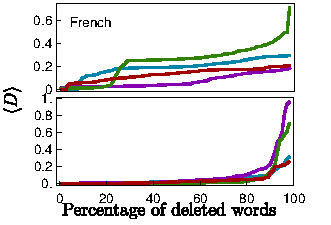
\includegraphics[scale=1.05]{ds2.pdf}};
    \node at (2*5.2,0)     {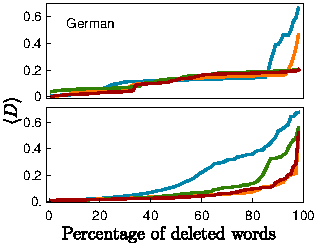
\includegraphics[scale=0.95]{ds3.pdf}};
    \node at (0,\tmp)      {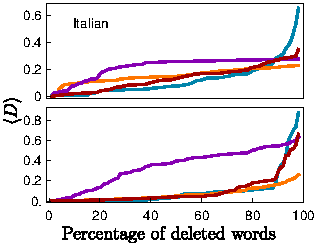
\includegraphics{ds4.pdf}};
    \node at (1*5.2,\tmp)  {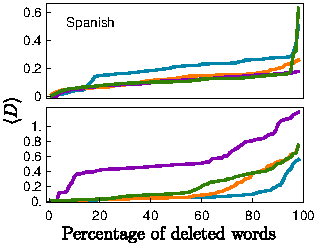
\includegraphics{ds5.pdf}};
    \node at (2*5.2,\tmp)  {
\includegraphics[scale=1.2]{prevolucion_legendas.pdf}};
%     \node at (-3.2,.65+3*0.35) [anchor=west] {\footnotesize Random two body};
%     \node at (-3.2,.65+2*0.35) [anchor=west] {\footnotesize $p=0.4$};
%     \node at (-3.2,.65+1*0.35) [anchor=west] {\footnotesize $p=0.99$};
%     \node at (-3.2,.65) [anchor=west] {\footnotesize $p=0.99$};
%   \node[rotate=90] at (-3.35,-1.6) {$\widetilde{Z}_Q^{\textbf{P}}$};
% \node[anchor=west] at (-3.5,0) {\footnotesize \marksymbol{square*}{red} Chain};
% \node[anchor=west] at (-3.5,-.5) {\footnotesize \marksymbol{square*}{green} Two body (o alrevez, checar)};
% \node[anchor=west] at (-3.5,-1) {\footnotesize \marksymbol{square*}{blue} General};
% \node[anchor=west] at (-2.45,1.7) {\tiny \marksymbol{square*}{black!45!green} Chain};
%   \node[anchor=west] at (-2.45,1.45) {\tiny \marksymbol{triangle*}{magenta} RSM $n_{\text{ens}}=1000$};
%   \node[anchor=west] at (-2.45,1.2) {\tiny \marksymbol{*}{black!50!green!10!cyan} RESM $n_{\text{ens}}=1$};
%   \node[anchor=west] at (-2.45,0.95) {\tiny \marksymbol{diamond*}{red} RESM $n_{\text{ens}}=10$};
%   \node[anchor=west] at (-2.45,0.70) {\tiny \hspace{.2cm} $\widetilde{Z}_Q^{\textbf{P}}$};
%   \node[anchor=west] at (-3, 2.5) {$(a)$};
%   \node[rotate=90] at (-3.35,-0.3) {RESM-10,};
%   \node[rotate=90] at (-3.35,1.4) {RESM-1};
%   \node[rotate=90] at (2.8,-0.55) {RSM-1000,};
%   \node[rotate=90] at (2.8,1.15) {RSM-10};
%   \node[rotate=90] at (-3.35, -1.2) {\marksymbol{diamond*}{red}};
%   \node at (-3.35, 0.65) {\marksymbol{*}{black!50!green!10!cyan}};
%   \node[rotate=90] at (2.8, -1.5) {\marksymbol{triangle*}{magenta}};
%   \node at (2.8, 0.4) {\marksymbol{square*}{black!45!green}};
%    \begin{scope}
%        \filldraw[thick,blue] (-2.35,0.70) -- (-2.35+0.2,0.70);
%    \end{scope}
\end{tikzpicture}
\end{document}
